%! Tex program = xelatex   
\documentclass{article}
\usepackage[left=2cm, right=2cm, lines=45, top=0.8in, bottom=0.7in]{geometry}
\usepackage{xeCJK}
\usepackage{amsmath}
\usepackage{booktabs} %表格
\usepackage{graphicx,subfig}
\setmainfont{Times New Roman}
\setCJKmainfont{Songti SC}
\setCJKfamilyfont{song}{Songti SC}
\renewcommand{\baselinestretch}{1.5} %行间距
%-----------------------伪代码------------------
\usepackage{algorithm}  
\usepackage{algorithmicx}  
\usepackage{algpseudocode}  
\floatname{algorithm}{Algorithm}  
\renewcommand{\algorithmicrequire}{\textbf{Input:}}  
\renewcommand{\algorithmicensure}{\textbf{Output:}} 
\usepackage{lipsum}  
\makeatletter
\newenvironment{breakablealgorithm}
  {% \begin{breakablealgorithm}
  \begin{center}
     \refstepcounter{algorithm}% New algorithm
     \hrule height.8pt depth0pt \kern2pt% \@fs@pre for \@fs@ruled
     \renewcommand{\caption}[2][\relax]{% Make a new \caption
      {\raggedright\textbf{\ALG@name~\thealgorithm} ##2\par}%
      \ifx\relax##1\relax % #1 is \relax
         \addcontentsline{loa}{algorithm}{\protect\numberline{\thealgorithm}##2}%
      \else % #1 is not \relax
         \addcontentsline{loa}{algorithm}{\protect\numberline{\thealgorithm}##1}%
      \fi
      \kern2pt\hrule\kern2pt
     }
  }{% \end{breakablealgorithm}
     \kern2pt\hrule\relax% \@fs@post for \@fs@ruled
  \end{center}
  }
\makeatother
%------------------------代码-------------------
\usepackage{xcolor} 
\usepackage{listings} 
\usepackage{fontspec}
\newfontfamily\menlo{Menlo}
\setmonofont[Mapping={}]{Monaco} 
\definecolor{mygreen}{rgb}{0,0.6,0}
\definecolor{mygray}{rgb}{0.5,0.5,0.5}
\definecolor{mymauve}{rgb}{0.58,0,0.82}
\lstset{ %
backgroundcolor=\color{white},   % choose the background color
basicstyle=\footnotesize\ttfamily,        % size of fonts used for the code
columns=fullflexible,
breaklines=true,                 % automatic line breaking only at whitespace
captionpos=b,                    % sets the caption-position to bottom
tabsize=4,
commentstyle=\color{mygreen},    % comment style
escapeinside={\%*}{*)},          % if you want to add LaTeX within your code
keywordstyle=\color{blue},       % keyword style
stringstyle=\color{mymauve}\ttfamily,     % string literal style
frame=single,
rulesepcolor=\color{red!20!green!20!blue!20},
numbers=left,
 numberstyle=\tiny\menlo
% identifierstyle=\color{red},
% language=c++,
}
\begin{document}
\title{计算机网络书面作业二}
\author{朱浩泽 1911530}
\maketitle
\section*{题目}
下图给出了一个包含两个自治域AS1和AS2的互联网拓扑结构,R2和R3为运行BGP协议的边界路由器,R1和R4分别为AS1和AS2的自治域内路由器(只运行自治域内路由协议OSPF),H1和H2为两台主机。假设每个物理网络都为以太网,每个接口的MAC地址用MACx的形式标在图中。请回答下列问题(所有IP地址和网络掩码使用点分十进制方法表示):
\begin{figure}[H]
    \centering
    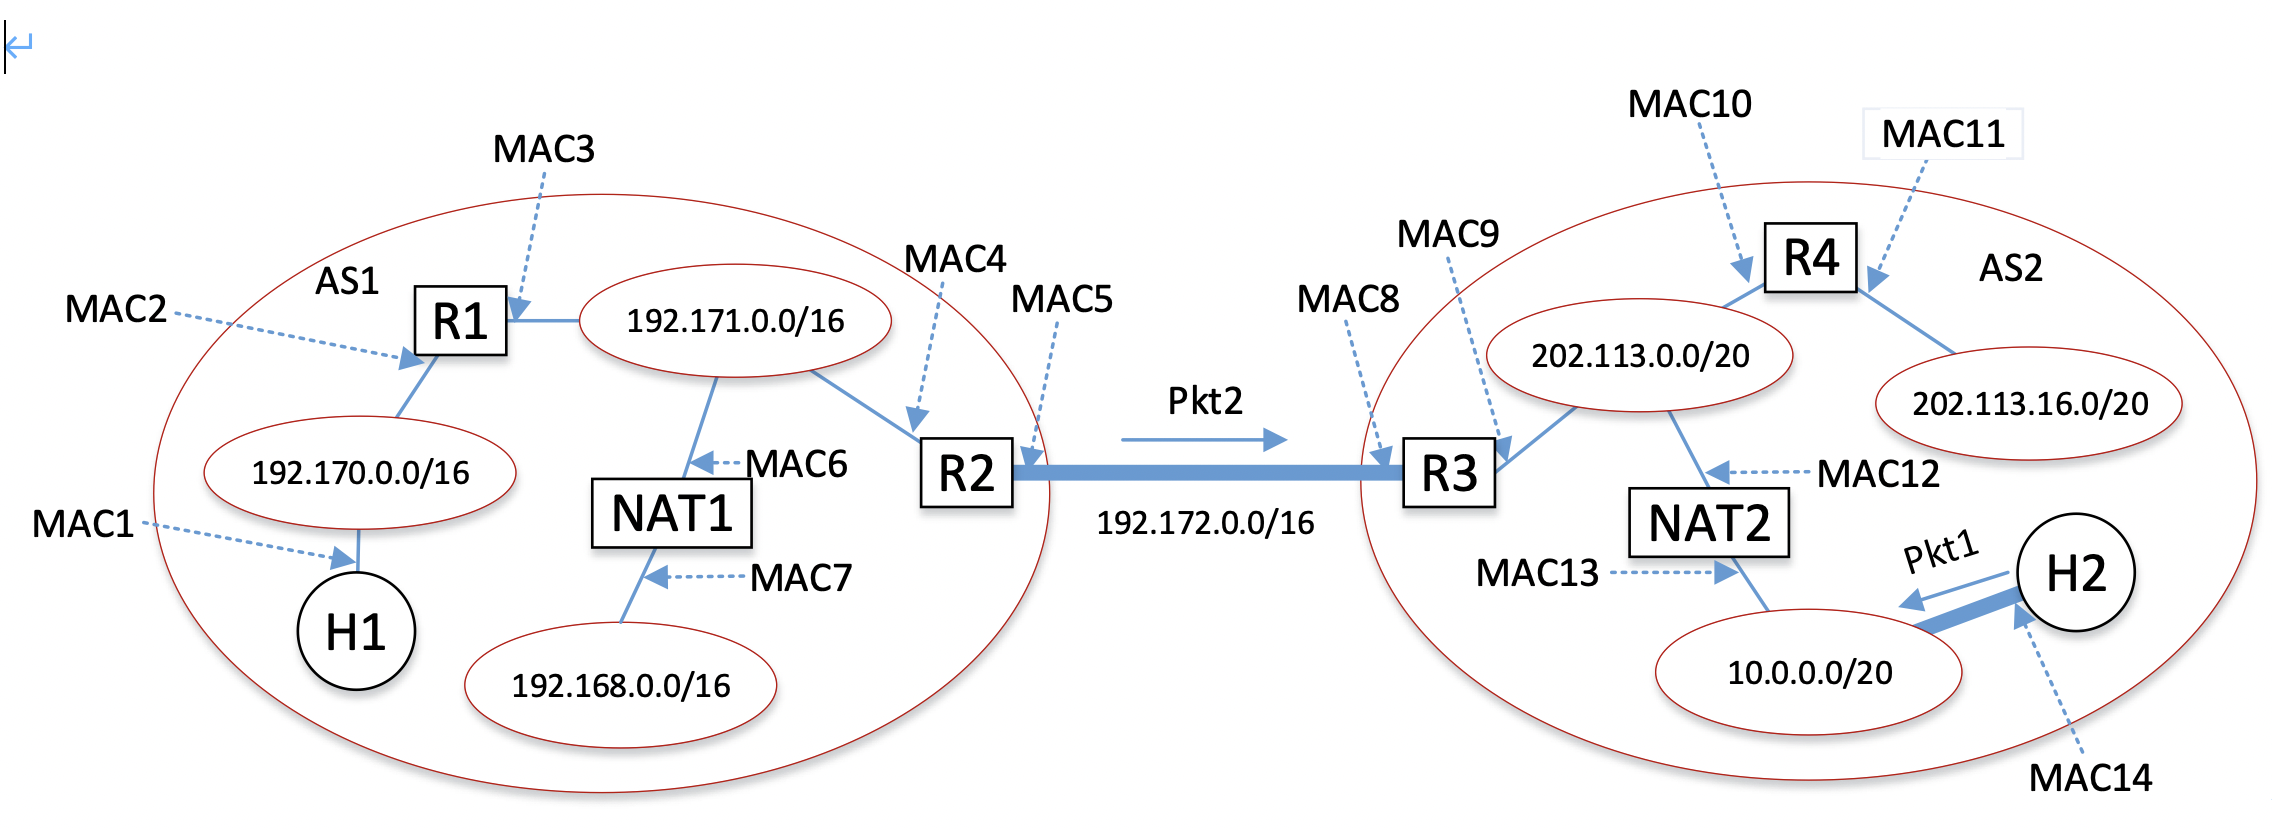
\includegraphics[scale=0.4]{1.png}
\end{figure}
\subsection{请根据网络拓扑结构图中给出的每个网络前缀为所有接口分配IP地址,并将分配的IP地址填写在下表中相应的位置(与MAC地址对应,无需标注网络掩码)。}
\begin{table}[!htbp]
  \centering
  \begin{tabular}{ccccccccccc}
  \toprule  
  接口MAC地址&分配IP地址& 接口MAC地址& 分配IP地址\\
  \midrule
  MAC1&192.170.0.1/16 & MAC8&192.172.0.2/16 \\
  MAC2&192.170.0.2/16 & MAC9&202.113.0.1/20\\
  MAC3&192.171.0.1/16 & MAC10&202.113.0.2/20 \\
  MAC4&192.171.0.2/16 & MAC11&202.113.16.1/20 \\
  MAC5&192.172.0.1/16 & MAC12&202.113.0.3/20 \\
  MAC6&192.171.0.3/16 & MAC13&10.0.0.1/20\\
  MAC7&192.168.0.1/16 & MAC14&10.0.0.2/20 \\
  \bottomrule
  \end{tabular}
\end{table}
\subsection{如果使用CIDR路由机制,边界路由器R2和R3相互通告怎样的网络可达信息(使边界路由器中保留的路由表项最少)。}
\ \ \ \ \ \ R2通告给R3:<AS1, 192.170.0.0/15>\\
\par R3通告给R2:<AS2, 202.113.0.0/19>
\subsection{根据给出的网络拓扑结构,在下面两个表中填写稳态情况下路由器R1和R3的路由表项(要求保留尽可能少的路由表项,且所有网络均可达)。}
\begin{table}[!htbp]
  \centering
  \begin{tabular}{ccccccccccc}
  \toprule  
  网络前缀&网络掩码& 下一步跳IP地址& 跳步数\\
  \midrule  
  192.170.0.0/16&255.255.0.0 & - &1\\
  192.171.0.0/16&255.255.0.0 & - &1\\
  192.172.0.0/16&255.255.0.0 & 192.170.0.2/16 &2\\
  202.113.0.0/19&255.255.224.0& 192.170.0.2/16 &3 \\
  \bottomrule
  \end{tabular}
  \caption{R1路由表}
\end{table}
\begin{table}[!htbp]
  \centering
  \begin{tabular}{ccccccccccc}
  \toprule  
  网络前缀&网络掩码& 下一步跳IP地址& 跳步数\\
  \midrule
  192.172.0.0/16&255.255.0.0 & -&1 \\
  192.170.0.0/15&255.254.0.0 & 192.172.0.1/16&2\\
  202.113.0.0/20&255.255.240.0 & -&1 \\
  202.113.16.0/20&255.255.240.0 & 202.113.0.2/20&2 \\
  \bottomrule
  \end{tabular}
  \caption{R3路由表}
\end{table}
\subsection{由主机H2发起,与主机H1建立一个TCP连接,两端使用的TCP端口分别为5050和80。图中给出了两个数据包Pkt1和Pkt2经过的链路和传输方向(经过的链路已加粗),请完成下面两个表的填写,给出每层数据单元头部中的源地址(或端口)和目的地址(或端口),并写出NAT2中的地址转换表(用表格形式给出)。(NAT设备的TCP端口由你自己分配)}
\begin{table}[!htbp]
  \centering
  \begin{tabular}{ccccccccccc}
  \toprule  
  数据包头类型&源地址(或端口)& 目的地址(或端口)\\
  \midrule
  以太头& MAC14& MAC13\\
  IP头& 10.0.0.2/20& 192.170.0.1\\
  TCP头& 5050& 80\\
  \bottomrule
  \end{tabular}
  \caption{数据包Pkt1}
\end{table}
\begin{table}[!htbp]
  \centering
  \begin{tabular}{ccccccccccc}
  \toprule  
  数据包头类型&源地址(或端口)& 目的地址(或端口)\\
  \midrule
  以太头& MAC5&MAC8 \\
  IP头& 192.172.0.1/16& 202.113.0.3/20\\
  TCP头&80 &  8080\\
  \bottomrule
  \end{tabular}
  \caption{数据包Pkt2}
\end{table}
\begin{table}[!htbp]
  \centering
  \begin{tabular}{ccccccccccc}
  \toprule  
  互联网侧&本地网络侧\\
  \midrule
  202.113.0.3,\ 8080 &10.0.0.2,\ 5050\\
  \bottomrule
  \end{tabular}
  \caption{NAT2中地址转换表}
\end{table}
\end{document}
